\chapter{Study 3}
\chaptermark{Study 3}
\label{ch:study3}
%\setcounter{equation}{0}

\newpage
%Abstract


% ====================================================================================================================
\section{Introduction}
\label{study3:intro}

% ==========================================================================================================

\section{Method}
\label{study3:method}
\subsection{Participants}
\label{study3:method:a}
Two hundred and seven healthy participants were recruited from the University of York (132 females, 65 males; age range = 18–-31 years, \textit{M} = 20.21, \textit{SD} = 2.36). 
This analysis included two data sets with some shared measurements and same MRI protocol as \ref{ch:study1}. 
Participants were right-handed native English speakers with normal or corrected-to-normal vision and no history of psychiatric or neurological illness. Participants underwent MRI scanning, completed an 1-hr online questionnaire. The first cohort is identical to the sample in \ref{ch:study1}. Participant attended three 
(165 participants; 99 females, 66 males; age range = 18–-31 years, \textit{M} = 20.43, \textit{SD} = 2.63) 2-hr behavioral testing sessions to complete a battery of cognitive tasks. 
The second cohort (42 participants; 33 females, 9 males; age range = 18–-23 years, \textit{M} = 19.79, \textit{SD} = 1.37) underwent two 2-hr behavioural testing sessions to complete a battery of cognitive tasks. The behavioural sessions took place within a week of the scan. Ten participants were excluded from the multivariate pattern analysis because they failed to complete all of the behavioural testing sessions. In total, 197 participants (126 females, 71 males; age range = 18–-31 years, \textit{M} = 20.11, \textit{SD} = 2.24) were included in the multivariate pattern analysis and the comparison with cognitive performance. Participants were rewarded with either a payment of \pounds 10 per hour or a commensurate amount of course credit. All participants provided written consent prior to the fMRI session and the first behavioural testing session. Approval for the study was obtained from the ethics committee of the University of York Department of Psychology and the University of York Neuroimaging Centre.

\subsection{MRI acquisition}
\label{study3:method:b}
The MRI acquisition protocol was identical to Chapter \ref{ch:study1}. Please refer to section \ref{study1:method:b} for details.

\subsection{Resting state data preprocessing}
\label{study3:method:c}

All preprocessing and denoising steps for the MRI data were carried out using the SPM software package (Version 12.0) and Conn functional connectivity toolbox (Version 17.f), based on the MATLAB platform (Version 17.a). The first three functional volumes were removed in order to achieve steady state magnetisation. The remaining data was first corrected for motion using six degrees of freedom (x, y, z translations and rotations), and adjusted for differences in slice-time. Subsequently, the high-resolution structural images were co-registered to the mean functional image via rigid-body transformation, segmented into grey/white matter and cerebrospinal fluid probability maps, and all functional volumes were spatially normalized to Montreal Neurological Institute (MNI) space using the segmented images and a priori templates. This indirect procedure utilizes the unified segmentation–normalization framework, which combines tissue segmentation, bias correction, and spatial normalization in a single unified model. No smoothing was employed, complying with recent studies that report the negative influence of this procedure on the construction of connectivity matrices analysis. 

Moreover, a growing body of literature indicates the potential influence of participant motion inside the scanner on the subsequent estimates of functional connectivity. In order to ensure that motion and other artefacts did not confound our data, we have employed an extensive motion-correction procedure and denoising steps, comparable to those reported in the literature. In addition to the removal of six realignment parameters and their second-order derivatives using the general linear model (GLM), a linear detrending term was applied as well as the CompCor method that removed five principle components of the signal from white matter and cerebrospinal fluid. Moreover, the volumes affected by motion were identified and scrubbed based on the conservative settings of motion greater than 0.5 mm and global signal changes larger than z = 3. Though recent reports suggest the ability of global signal regression to account for head motion, it is also known to introduce spurious anti-correlations, and was thus not utilised in our analysis. Finally, a band-pass filter between 0.009 Hz and 0.08 Hz was employed in order to focus on low frequency fluctuations.

\subsection{ROI-ROI functional connectivity.}
\label{study3:method:d}
We adopted a set of 57 regions based on the Yeo 7 networks. We split the networks into two hemispheres and extracted clusters. Two voxels are considered connected only if they are adjacent within the same x, y, or z direction. This yielded 57 clusters from the Yeo 7 networks parcellation. The implementation of spatial clusters extraction was retrieved from python library Nilearn \cite[ \url{http://nilearn.github.io/}, version 0.3.1]{Abraham2014}. Fully-connected, undirected and weighted matrices of bivariate correlation coefficients (Pearson's r) were constructed for each participant using the average BOLD signal time series obtained from all the 57 ROIs described above. The off-diagonal of each correlation matrix contained 1596 unique region-region connection strengths (i.e., the upper or lower triangle of the network covariance matrix). This approach provided a measure of connection strength of the whole brain for each participant. Finally, Fisher’s r-to-z transformation was applied to each network covariance matrix. 

\subsection{Behavioural data}
\label{study3:method:e}

\subsubsection{Cognitive tasks}
We selected 9 cognitive tasks that are common across the two cohorts. The selected tasks measures cognitive functions that have been examined in previous mind-wandering literature, encompassing executive control (digit span, task switching task), generation of information (unusual uses task, verbal fluency task), semantic memory (semantics relatedness judgement tasks, feature matching task), episodic memory (paired associate task, four mountains task), and fluid intelligence (Raven Advanced Progressive Matrices; RAPM). Thirteen cognitive scores were calculated from the selected tasks. Please refer to Appendix \ref{appendix:study1:subsection2} for the detailed description of the tasks. 

\subsubsection{Experience sampling}
Please refer to Chapter \ref{ch:study1} section \ref{study1:method:d} for the experience sampling data collection and Table \ref{tab:study1:1} for the detailed questions. 


\subsection{Multivariate pattern analysis}
\label{study3:method:f}
\subsubsection{SCCA}
We performed a sparse canonical correlation analysis \cite<SCCA; see>{Hastie2015}%{ Hastie, Tibshirani, \& Wainwright, 2015} 
on the functional connectomes and the cognitive tasks, to yield latent components that reflect multivariate patterns across neural organisation and cognition \cite<For similar application, see>{Wang2018}%Wang et al., 2017). 
SCCA maximised the linear correlation between the low-rank projections of two sets of multivatiate data sets with sparse model to regularise the decomposition solutions a process that helps maximise the interpretability of the results. The regularisation function of choice is L1 penalty, which produces ‘sparse’ coefficients, meaning that the canonical vectors (i.e., translating from full variables to a data matrix’s low-rank components of variation) will contain a number of exactly zero elements. L1 regularisation conducted (i) feature selection (i.e., select only relevant components) and (ii) model estimation (i.e., determine what combination of components best disentangles the neuro-cognitive relationship) in an identical process. This way we handle adverse behaviours of classical linear models in high-dimensional data. A reliable and robust open-source implementation of the SCCA method was retrieved as R package from CRAN 
\cite<PMA, penalized multivariate analysis, version 1.0.9>{Witten2009a}%(PMA, penalized multivariate analysis, version 1.0.9, Witten, Tibshirani, \& Hastie, 2009).
The amount of L1 penalty for the functional connectomes and cognitive task performance were chosen by cross-validation. The procedure is described below. 

\subsubsection{Model Selection}
The model selection process was conducted with two parts: L1 penalty coefficient selection and component selection. For the L1 penalty coefficient selection, we performed a grid search combined with cross-validation (CV) to avoid over-fitting \cite{BzdokYeo2017}. 
Of each penalty pair on the search grid, a 10-fold cross-validation was performed to search for the best out-of-sample the rank-1 canonical correlation. We then decomposed the full dataset with the selected L1 penalty coefficients. The K-Fold CV was conducted by the implementation in Python library scikit-learn \cite<http://scikit-learn.org/stable/, version 0.18.2>{scikit-learn}. 

Confound removal was performed on the functional connectomes and the cognitive scores as suggested by prior study \cite{Smith2015}. 
The confound variables were sex, age, and head motion indicated by mean frame-wise displacement \cite{Jenkinson2002}.
The  removal  steps  was  performed  on  the training set in each CV fold. The z-scores of the confound variables were calculated, and also squared the three confound measures to account for potentially nonlinear effects of these confounds. The 6 resulting confounds were regressed out of both data matrices. 
The implementation of the confound removal method \cite{Friston1994} was retrieved from Python library Nilearn \cite[ \url{http://nilearn.github.io/}, version 0.3.1]{Abraham2014}.

After finding the optimal hyper-parameters, 1000 permutation tests with family-wise error correction was applied to access the component(s) that occur above chance. We constructed a null distribution for each canonical component by holding the functional connectivity data in place and randomising the row order of self-reports data. This permutation scheme broke the link of individual differences in the dataset, therefore testing the robustness of the components in the hypothetical population. By calculating the false-discovery rate in the null distribution, we can conclude the possibility of discovering our components by chance with the given penalty coefficients. Hypotheses that are accepted with a 5\% level of significance. In the current analyses we adopt the permutation test with the FWE-corrected p-value by Smith and colleagues \citeyear{Smith2015}. All components were compared to the first sparse canonical correlation of the permuted sample. The low-rank components are more relevant that the rest, therefore we yield more conservative p-value by comparing to the first canonical correlation only. 

\subsection{Group analysis}
\label{study3:method:g}

To determine how patterns of unconstrained neuro-cognitive activity related to performance on the self-report experience, we conducted an independent statistical analysis on the identical subjects. A Type III multivariate multiple regression with Pillai's trace test was applied to 5 individual scores for each of the latent components describing the neuro-cognitive mechanism from the SCCA were the independent variables, and the 13 measures from MDES were the dependent variables that we hoped to described by the linear combination of the latent components. Pillai's trace test is considered to be the most powerful and robust statistic for general use \cite{Huberty2006}.
The p-values reported were based on Bonferroni correction. The analysis was conducted in R (version 3.3.1). The multivariate multiple regression was conducted in R (version 3.3.1) using function ‘Manova’ in R package ‘car’ (companion to applied regression, version 2.1–5).

% ==========================================================================================================
\section{Results}
\label{study3:results}

\subsection{Determining constituent category of cognitive functions}

\begin{wrapfigure}{i}{0.35\textwidth}    
    \vspace{-20pt}
    \centering
    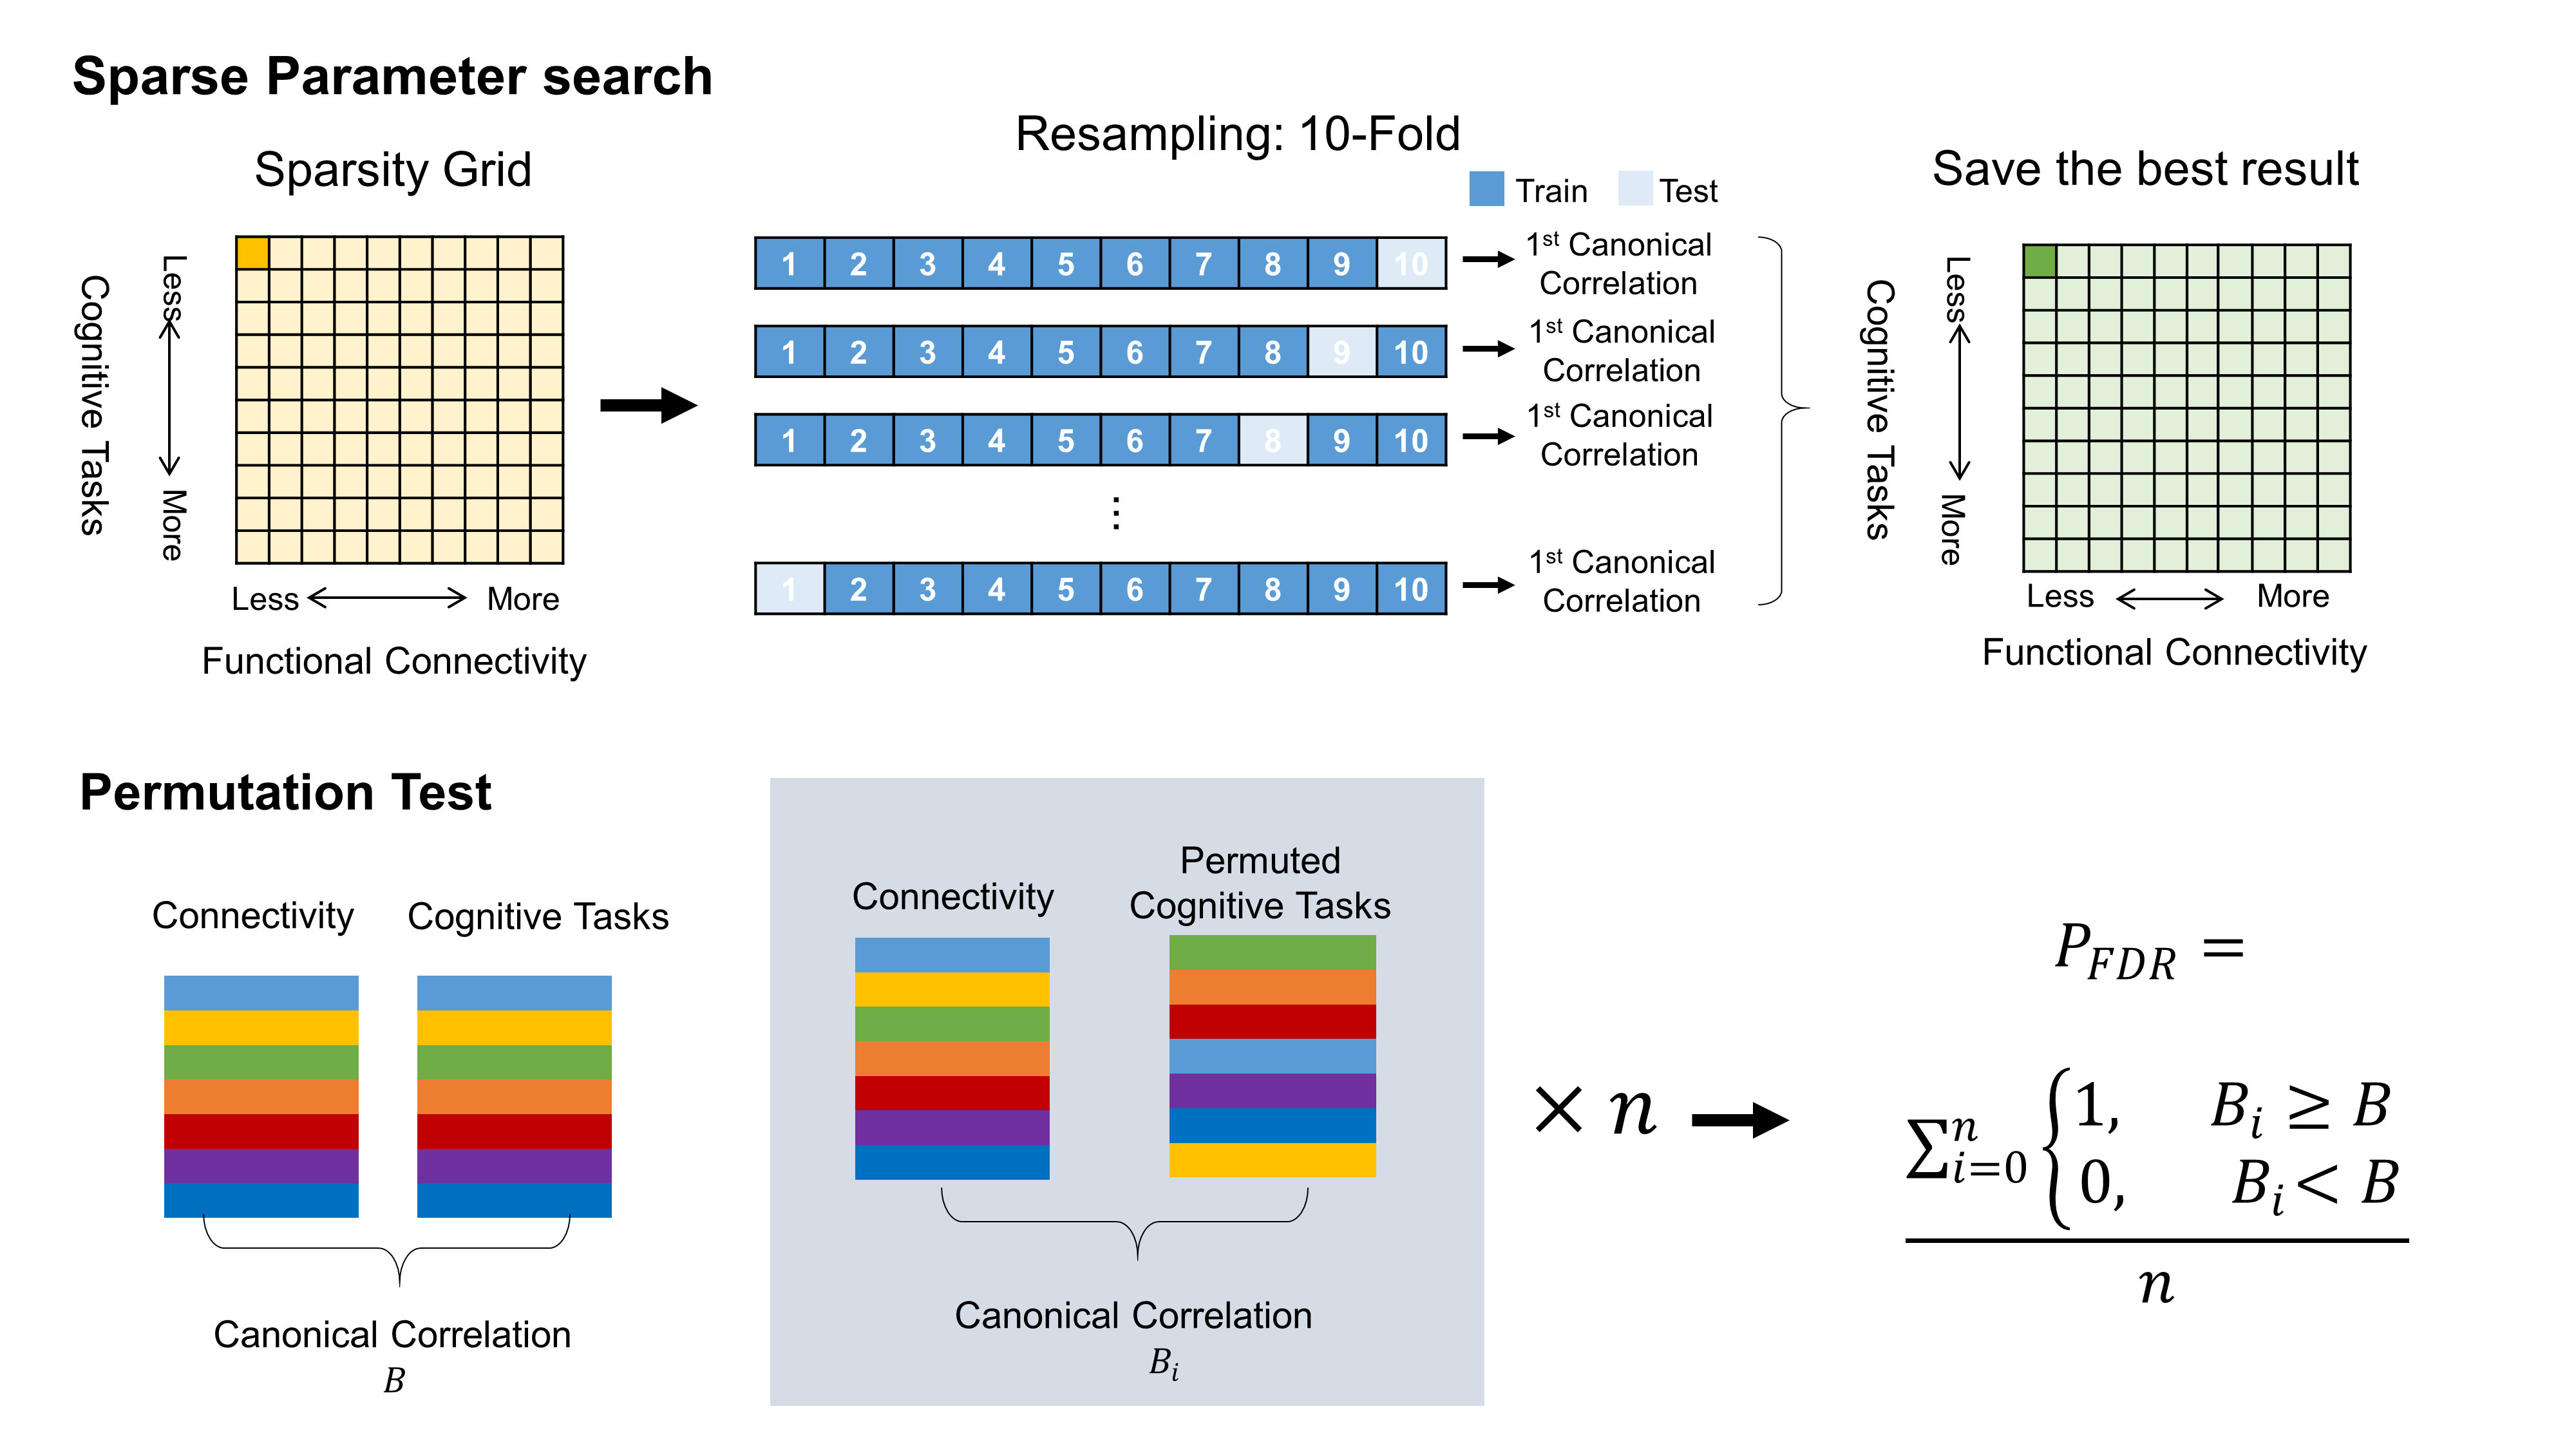
\includegraphics[width=0.33\textwidth]{chapters/img/study3fig1.png}
	\caption{Grid search.} 
	\label{fig:study3:fig1}
	\vspace{-20pt}
\end{wrapfigure}

Sparse Canonical Correlation Analysis (SCCA) was used to determine connectome-wide dimensions that describe common variance shared by descriptions of brain and experience. This took as input individual scores for the connections between each of the regions extracted from Yeo’s 7 networks parcellation and the 13 cognitive task scores.

We applied SCCA with 10-fold CV and permutation tests as the model selection strategy. We obtained penalty levels of 0.6 on both the functional connectivity and cognitive tasks indicated the best out-of-sample prediction on our data through the grid search (Figure \ref{fig:study3:fig1}). Five significant canonical components was identified through FWE-corrected p-value through permutation tests. The p-values of the 5 components are x, x, x, x, x. The canonical correlations of the 5 latent components were a, b, c, d, and e. Since the sparsity turns CCA into a convex optimisation problem, the modes didn't come out in the descending order of their canonical correlations. The latent components yielded by the best model are presented in Figure \ref{fig:study3:fig2}. For the ease of presentation and interpretation, we summarized the components as network-network connectivity instead of 57-by-57 connectivity matrices. The heat maps describe the network-to-network correlations and the cognitive tasks. 

\begin{figure}[H]
    \vspace{-10pt}
	\centering
	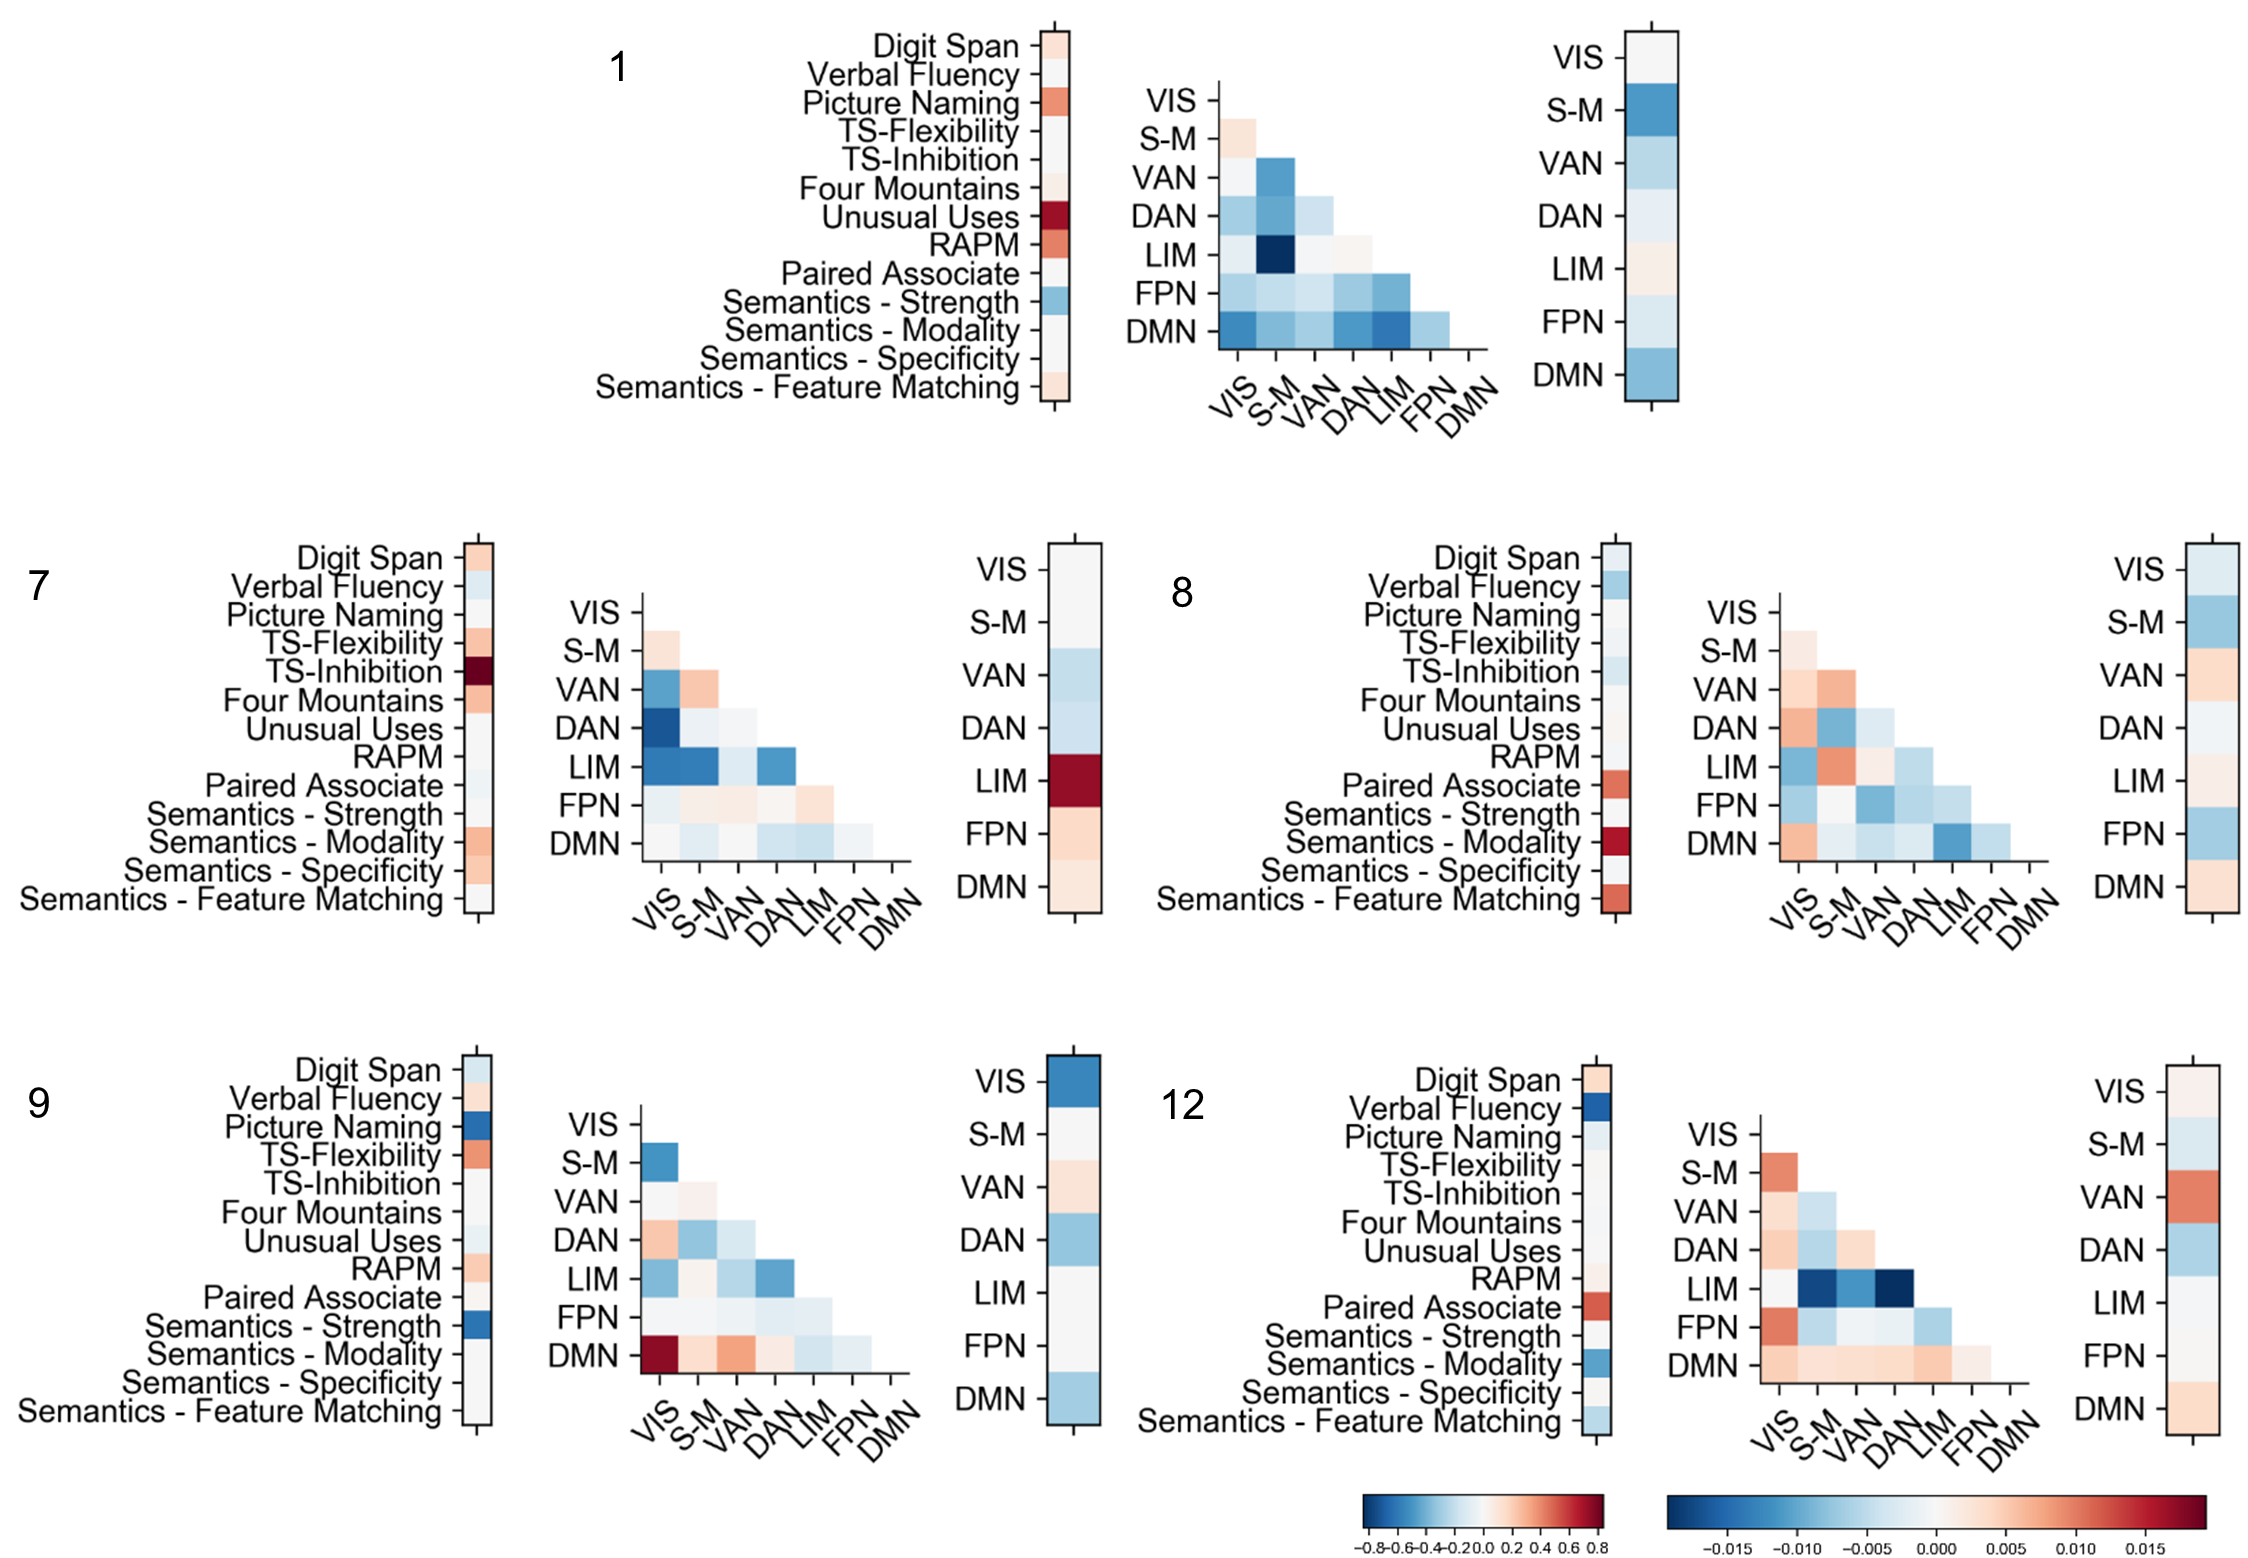
\includegraphics[width=1\textwidth]{chapters/img/study3fig2.png}
	\caption{Significant components.} 
	\caption*{
	\footnotesize{
	}
	}
	\label{fig:study3:fig2}
	\vspace{-20pt}
\end{figure}

% explain the significant components
Component 1 - semantic control is relevant, along with intelligence, and being able to name pictures

Component 7 -  maintaining a pattern of ongoing thought that is relatively pristine in its nature that is free from other irrelevant sources of information

Component 8 - cognitive control, pitting exec tasks against more automatic semantic retrieval. So people who have better control think less detailed past thoughts? 

Component 9 -  mental imagery vs. verbal fluency?

Component 12 - episodic vs. verbal semantic.

\subsection{The relationship between neuro-cognitive components and self-reports on thoughts}
% multivariate main effect
Three regression models were performed to evaluate the relationship between neuro-cognitive components and self-reports on thoughts: average scores of all thought probes, thought probes in 0-back and 1-back conditions. In the model of all thought probes, we got multivariate main effect in component 7 and 12. In the 0-back condition, only component 7 showed the main effect in multivaraite level. The 1-back condition model showed significant results in component 7 and component 12. 
\begin{figure}[H]
	\centering
	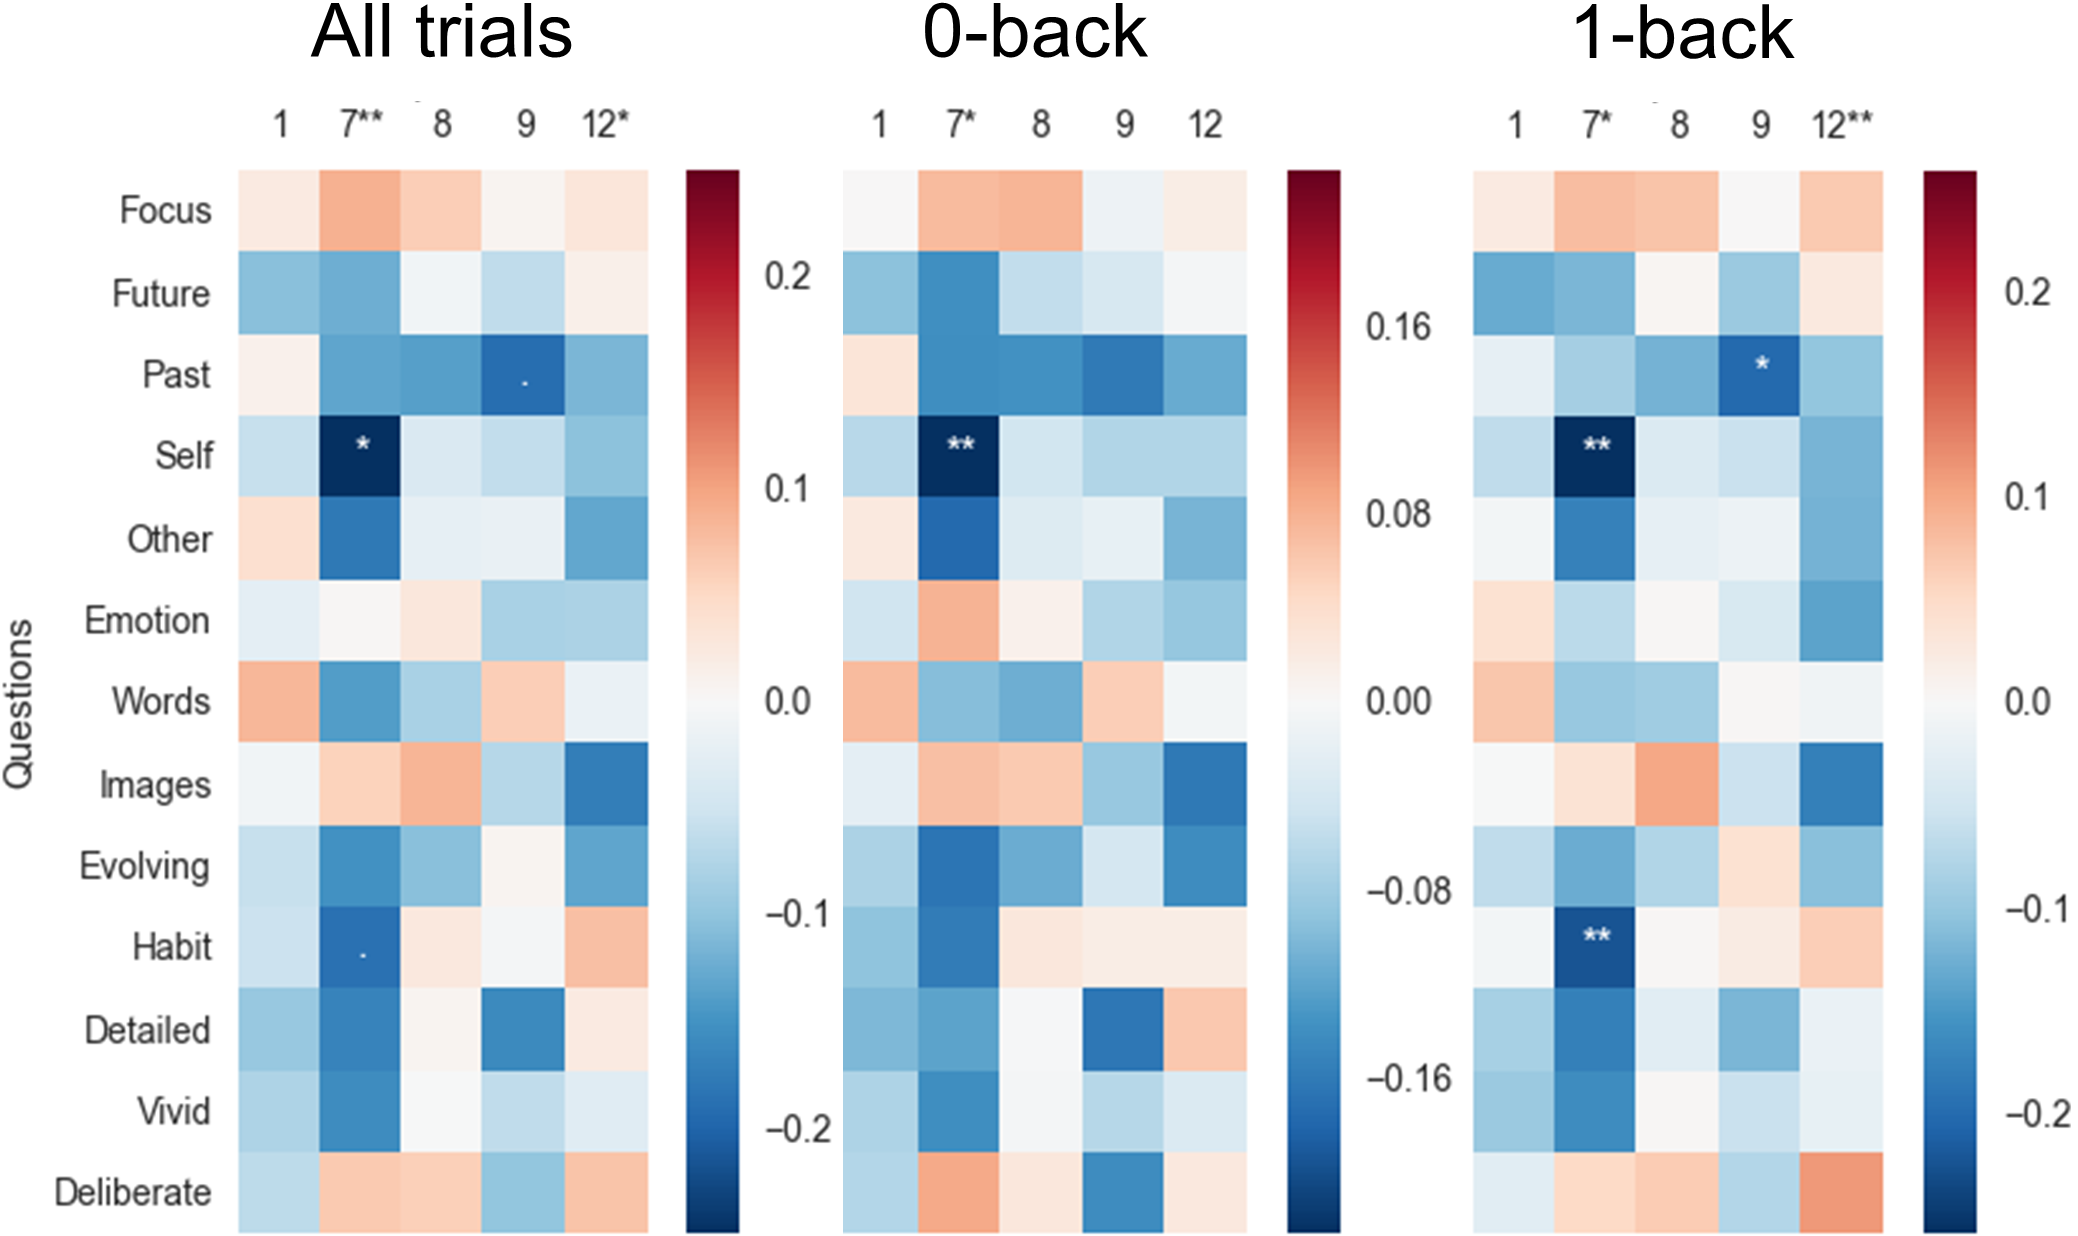
\includegraphics[width=0.8\textwidth]{chapters/img/study3fig3.png}
	\caption{Univariate results.} 
	\caption*{
	\footnotesize{
	}
	}
	\label{fig:study3:fig3}
\end{figure}


% ==========================================================================================================
\newpage
\section{Discussion}
\label{study3:discussion}
